\section{Linear regression}

The goal of regression is to approximate a function $f(x)$ that maps input $x$ to a continuous output $t$ from a dataset $\mathcal{D}$: 
\[\mathcal{D}=\left\{ \left\langle x,t \right\rangle \right\} \implies t=f(x)\]
Here, $x$ is a vector. 
To perform regression, we assume the existence of a function capable of performing this mapping.
The key components of constructing a linear regression problem include:
\begin{itemize}
    \item The method used to model the function $f$ (the hypothesis space). 
    \item The evaluation criteria for the approximation (the loss function).
    \item The optimization process for optimizing the model.
\end{itemize}

In linear regression, the function $f$ is modeled using linear functions. 
This choice is motivated by several factors:
\begin{itemize}
    \item Linear models are easily interpretable, making them suitable for explanation.
    \item Linear regression problems can be solved analytically, allowing for efficient computation.
    \item Linear functions can be extended to model nonlinear relationships.
    \item More sophisticated methods often build upon or incorporate elements of linear regression.
\end{itemize}

\paragraph*{Hypothesis space}
In mathematical terms, the approximation $y$ can be defined as: 
\[y(\textbf{x},\textbf{w})=w_0+\sum_{j=1}^{D-1}w_j x_j=\textbf{w}^T\textbf{x}\]
Here, $\textbf{x} = \left( 1,x_1,\dots,x_{D-1} \right)$ is a vector, and $w_0$ is called the bias parameter.
It's important to note that the output $y$ is a scalar value. 

In a two-dimensional space, our hypothesis space will be the set of all points in the plane $(w_0,w_1)$. 
The coordinates of each point will correspond to a line in the $\left( \textbf{x}, y \right)$ space.

\paragraph*{Loss function}
A commonly used error loss function for the linear regression problem is the sum of squared errors (SSE), defined as:
\[L(\textbf{w})=\dfrac{1}{2}\sum_{n=1}^{N}\left( y(x_n, \textbf{w})-t_n \right)^2\]
This sum is also referred to as the residual sum of squares (RSS) and can be expressed as the sum of squared residual errors:
\[RSS(\textbf{w})=\left\lVert \boldsymbol{\epsilon}^2_2 \right\rVert = \sum_{i=1}^{N}\epsilon^2_i \]
This formulation of the loss function allows for obtaining a closed-form optimization solution.

\paragraph*{Optimization}
For linear models, a closed-form optimization of the RSS, known as least squares, begins with the matrix representation of the loss function:
\[L(\textbf{w})=\dfrac{1}{2}RSS(\textbf{w})=\dfrac{1}{2}\left( \textbf{t}-\boldsymbol{\Phi}_{\textbf{w}} \right)^T\left( \textbf{t}-\boldsymbol{\Phi}_{\textbf{w}} \right)\]
Here, $\boldsymbol{\Phi}=\begin{bmatrix} \phi(x_1) & \dots & \phi(x_N)\end{bmatrix}^T$ and $\textbf{t}=\begin{bmatrix}t_1 & \dots & t_n\end{bmatrix}^T$.
To find the optimal $\textbf{w}$, we compute the first derivative of $L(\textbf{w})$ and set it to zero:
\[\hat{\textbf{w}}_{OLS}=\left( \boldsymbol{\Phi}^T\boldsymbol{\Phi}\right)^{-1}\boldsymbol{\Phi}^T\textbf{t}\]
However, the inversion of the matrix $\boldsymbol{\Phi}^T\boldsymbol{\Phi}^{-1}$ can be computationally expensive, especially for large datasets, with a complexity of $O(nm^2+m^3)$, assuming the matrix is non-singular (invertible). 

To mitigate this, stochastic gradient descent (SGD) can be employed. 
The algorithm known as least mean squares (LMS) uses the following update rule:
\[L(\textbf{x})=\sum_nL(x_n)\]
Expanding this, we get:
\begin{align*}
    \textbf{w}^{(n+1)}  &= \textbf{w}^{(n)}-\alpha^{(n)}\nabla L(x_n) \\
                        &= \textbf{w}^{(n)}-\alpha^{(n)}\left( \textbf{w}^{(n)^T}\phi(\textbf{x}_n)-t_n \right)\phi(\textbf{x}_n)
\end{align*}
Here, $\alpha$ is the learning rate, and convergence is guaranteed if $\sum_{n=0}^{\infty}=+\infty$ and $\sum_{n=0}^{\infty}=\alpha^{(n)^2}<+\infty$.

If the regression problem involves multiple outputs, meaning that $\textbf{t}$ is not a scalar, we can solve each regression problem independently.
However, we can still use the same set of basis functions.
The solution for the weight vectors for all outputs can be expressed as:
\[\hat{\textbf{W}}=\left( \boldsymbol{\Phi}^T\boldsymbol{\Phi}\right)^{-1}\boldsymbol{\Phi}^T\textbf{T}\]
Here, each column of matrix $\textbf{T}$ and $\hat{\textbf{W}}$ corresponds to the target vector and the weight vector for each output, respectively.
This solution can be easily decoupled for each output $k$: 
\[\hat{\textbf{w}}_k=\left( \boldsymbol{\Phi}^T\boldsymbol{\Phi}\right)^{-1}\boldsymbol{\Phi}^T\textbf{t}_k\]
An advantage of this approach is that $\left( \boldsymbol{\Phi}^T\boldsymbol{\Phi}\right)^{-1}$ only needs to be computed once, regardless of the number of outputs.

\subsection{Basis function}
While a linear combination of input variables may not always suffice to model data, we can still construct a regression model that is linear in its parameters. 
This can be achieved by defining a model using non-linear basis functions, expressed as:
\[y(\textbf{x},\textbf{w})=w_0+\sum_{j=1}^{M-1}w_j \phi_j(\textbf{x})=\textbf{w}^T\boldsymbol{\phi}(\textbf{x})\]
Here, the components of the vector  $\boldsymbol{\phi}(\textbf{x})=\left( 1,\phi_1(\textbf{x}),\dots,\phi_{M-1}(\textbf{x}) \right)^T$  are referred to as features.
These features allow for a more flexible representation of the input data, enabling the model to capture non-linear relationships between the input variables and the output.
\begin{example}
    Let's reconsider a set of data regarding individuals' weight and height, along with their completion times for a one-kilometer run:
    \begin{table}[H]
        \centering
        \begin{tabular}{c|c|c}
        \textbf{Height (cm)} & \textbf{Weight (kg)} & \textbf{Completion time (s)} \\ \hline
        180                  & 70                   & 180                          \\
        184                  & 80                   & 220                          \\
        174                  & 60                   & 170                         
        \end{tabular}
    \end{table}
    We can model this problem using a dummy variable and introduce the Body Mass Index (BMI) as a new feature:
    \begin{table}[H]
        \centering
        \begin{tabular}{c|c|c|c|c}
        \textbf{Dummy variable} & \textbf{Height (cm)} & \textbf{Weight (kg)} & \textbf{BMI} & \textbf{Completion time (s)} \\ \hline
        $x_0$                   & $x_1$                & $x_2$                & $x_3$        & $t$                          \\
        1                       & 180                  & 70                   & 21           & 180                          \\
        1                       & 184                  & 80                   & 23           & 220                          \\
        1                       & 174                  & 60                   & 20           & 170                         
        \end{tabular}
    \end{table}
    Here, the dummy variable $x_0$ is always initialized to one.
    Now, we have the option to retain or discard the weight and height variables, considering only the BMI values for analysis.
\end{example}
The most commonly used basis functions in regression are:
\begin{itemize}
    \item \textit{Polynomial}: 
        \[\phi_j(x)=x^j\]
    \item \textit{Gaussian}:
        \[\phi_j(x)=\exp \left( -\dfrac{\left( x-\mu_j \right)^2}{2 \sigma^2} \right) \]
    \item \textit{Sigmoidal}: 
        \[\phi_j(x)=\dfrac{1}{1+\exp\left(\dfrac{\mu_j-x}{\sigma}\right)}\]
\end{itemize}
Here, the constant $\mu_j$ is referred to as a hyperparameter, as its value needs to be determined through experimentation and depends on the user's experience.

\begin{figure}[H]
    \centering
    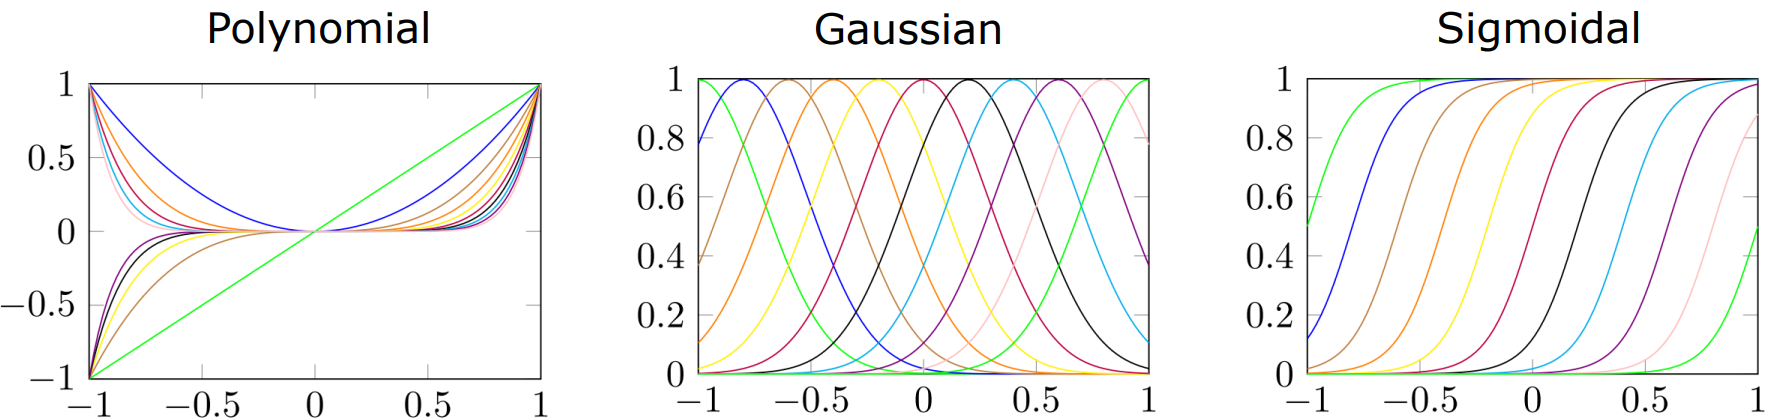
\includegraphics[width=0.75\linewidth]{images/basis.png}
    \caption{Some possible basis functions shapes}
\end{figure}

It's noteworthy that the Gaussian basis function allows for a local approximation by omitting values that are close to zero.
This approach enables capturing the relationship between the input and output in a reduced input space area.
As we move away from the mean, approaching zero, the values become negligible.

\subsection{Regularization}
A function can achieve a better approximation by increasing the degree of the polynomial used in the regression.
\begin{example}
    Consider a function generating a set of points with some noise:
    \begin{figure}[H]
        \centering
        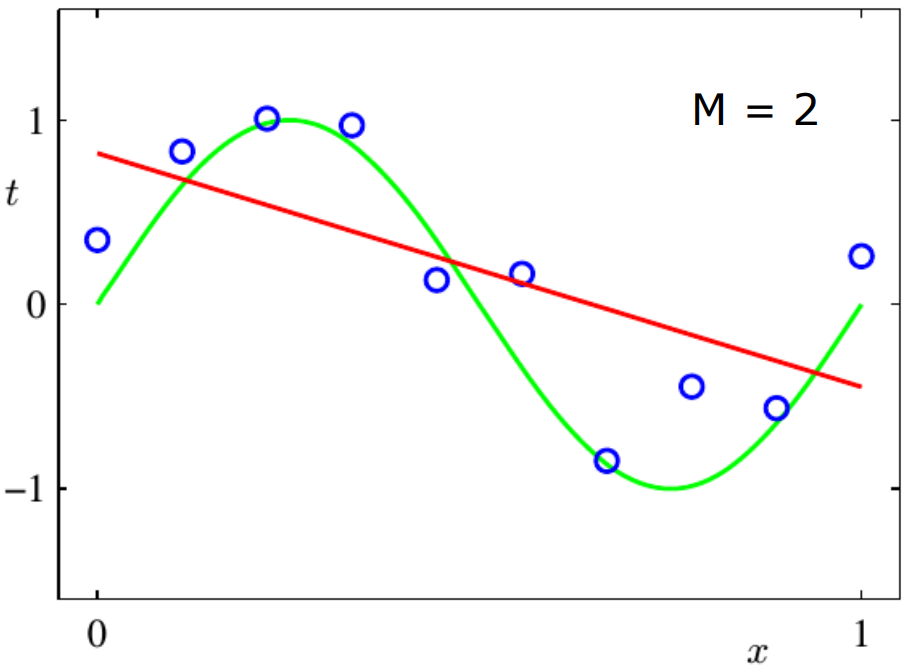
\includegraphics[width=0.25\linewidth]{images/reg.png}
    \end{figure}
    Using a second-order polynomial instead of a linear one provides a better approximation:
    \begin{figure}[H]
        \centering
        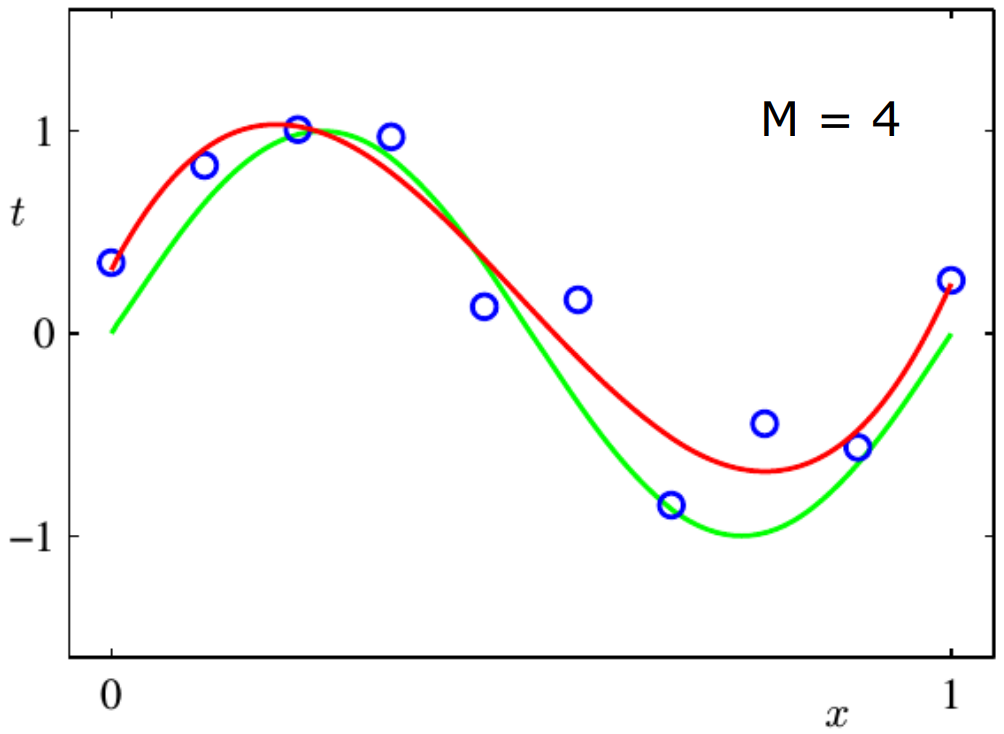
\includegraphics[width=0.25\linewidth]{images/reg1.png}
    \end{figure}
    Further improving the approximation can be achieved with a higher-degree polynomial (e.g., ninth grade):
    \begin{figure}[H]
        \centering
        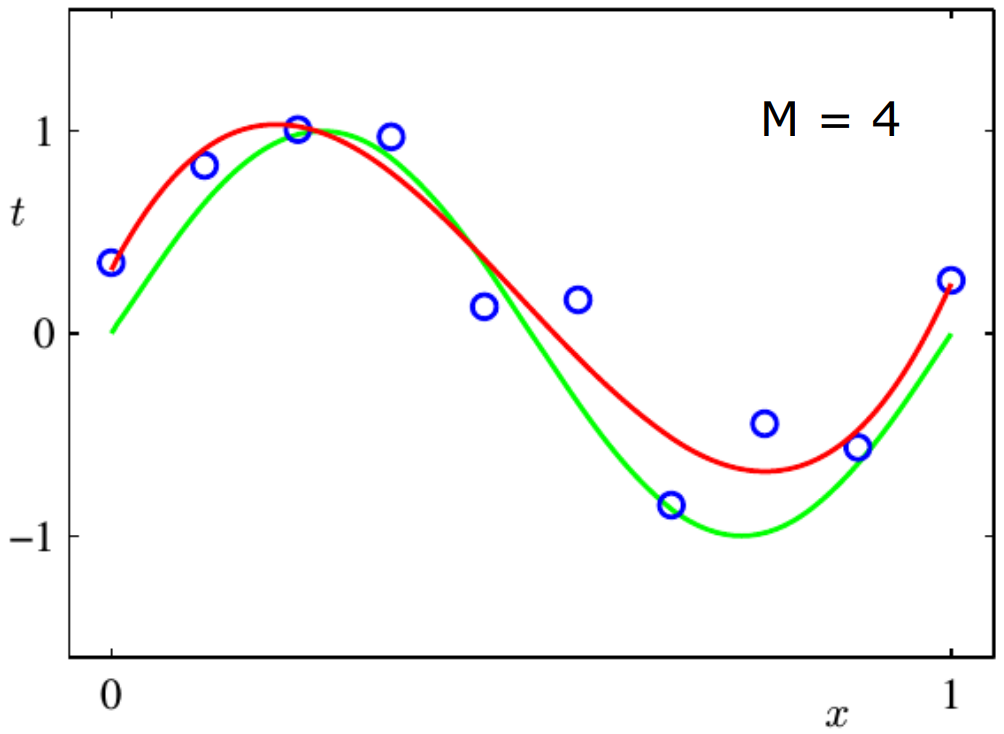
\includegraphics[width=0.25\linewidth]{images/reg1.png}
    \end{figure}
\end{example}
However, increasing the polynomial degree also increases the complexity of the model parameters.
To address this complexity, adjustments are needed in the loss function:
\[L(\textbf{w})=L_D(\textbf{w})+\lambda L_W(\textbf{w})\]
Here, $L_D(\textbf{w})$ represents the usual loss function, $L_W(\textbf{w})$ reflects model complexity (a hyperparameter), and $\lambda$ is the regularization coefficient.
$L_W(\textbf{w})$ can be tailored using ridge regression or lasso methods.

\paragraph*{Ridge regression}
In ridge regression, the regularization term $L_W(\textbf{w})$ is defined as:
\[L_W(\textbf{w})=\dfrac{1}{2}\textbf{w}^T\textbf{w}=\dfrac{1}{2}\left\lVert \textbf{w} \right\rVert_2^2 \]
Thus, the overall loss function becomes:
\[L(\textbf{w})=\dfrac{1}{2}\sum_{i=1}^N \left( t_i-\textbf{w}^T\phi(x_i) \right)^2 + \dfrac{\lambda}{2}\left\lVert \textbf{w} \right\rVert_2^2\]
Despite the regularization term, the loss function remains quadratic with respect to $w$, allowing for closed-form optimization:
\[\hat{\textbf{w}}_{ridge}=\left( \lambda\textbf{I}+\boldsymbol{\Phi}^T \boldsymbol{\Phi} \right)^{-1}\boldsymbol{\Phi}^T\text{t}\]
The term $\lambda\textbf{I}$ is crucial in solving the singularity problem, as it transforms a non-singular matrix into a singular one with an appropriate choice of $\lambda$. 

\paragraph*{Lasso}
Another common regularization method is lasso, where the regularization term $L_W(\textbf{w})$ is defined as:
\[L_W(\textbf{w})=\dfrac{1}{2}\left\lVert \textbf{w} \right\rVert_1=\dfrac{1}{2}\sum_{j=0}^{M-1}\left\lvert w_j \right\rvert\]
Thus, the overall loss function becomes:
\[L(\textbf{w})=\dfrac{1}{2}\sum_{i=1}^N \left( t_i-\textbf{w}^T\phi(x_i) \right)^2 + \dfrac{\lambda}{2}\left\lVert \textbf{w} \right\rVert_1\]
In this case, closed-form optimization is not possible. 
However, lasso typically leads to sparse regression models: when the regularization coefficient $\lambda$ is large enough, some components of $\hat{\textbf{w}}$ become equal to zero.
Regularization can be seen as equivalent to minimizing  $L_D(\textbf{w})$ subject to the constraint:
\[\sum_{j=0}^{M-1}\left\lvert w_j \right\rvert \leq \eta\] 

\subsection{Linear regression with probability}
We can approach regression in a probabilistic manner by defining a model that probabilistically maps inputs ($x$) to outputs ($t$).
This model, denoted as $y(x, w)$, incorporates unknown parameters ($w$).
We then model the likelihood, i.e., the probability that observed data $\mathcal{D}$ is generated by a given set of parameters ($w$), as: 
\[\text{P}(\mathcal{D}|\textbf{w})\]
Finally, we estimate the parameters ($w$) by maximizing the likelihood:
\[\textbf{w}_{ML}=\argmax_{\textbf{w}}\text{P}(\mathcal{D}|\textbf{w})\]

For linear regression, we define the model as:
\[t=y(\textbf{x},\textbf{w})+\epsilon=\textbf{w}^T\boldsymbol{\Phi}(\textbf{x})+\epsilon\]
Here, we assume a linear model for $y(\textbf{x},\textbf{w})$ and introduce noise  $\epsilon\sim\mathcal{N}(0,\sigma^2)$. 
Consequently, given a dataset $\mathcal{D}$ of $N$ samples with inputs $\textbf{X}=\begin{bmatrix}\textbf{x}_1 & \dots & \textbf{x}_n \end{bmatrix}$ and outputs $\textbf{t}=\begin{bmatrix}t_1 & \dots & t_n \end{bmatrix}^T$, we have: 
\[\text{P}(\mathcal{D}|\textbf{w})=\text{P}(\textbf{t}|\textbf{X},\textbf{w},\sigma^2)=\prod_{n=1}^{N}\mathcal{N}(t_n|\textbf{w}^T\boldsymbol{\Phi}(\textbf{x}_n),\sigma^2)\]
 
To find $\textbf{w}_{ML}$, it is convenient to maximize the log-likelihood, obtaining:
\[\ell (\textbf{w})=\ln\text{P}(t_n|\textbf{x}_n, \textbf{w} ,\sigma^2)=-\dfrac{N}{2}\ln(2\pi\sigma^2)-\dfrac{1}{2\sigma^2}RSS(\textbf{w})\]
Notice that the first part of the final formula is a constant independent of $\textbf{w}$, so it can be ignored in maximizing the likelihood.
Solving the optimization problem by setting the gradient to zero $\ell (\textbf{w})=0$, yields the final formula:
\[\textbf{w}_{ML}=\left( \boldsymbol{\Phi}^T\boldsymbol{\Phi} \right)^{-1}\boldsymbol{\Phi}^T\textbf{t}\]
This result aligns with the ordinary least squares approach.

This outcome allows us to interpret ordinary least squares from a probabilistic perspective, confirming that we are utilizing a normally distributed probabilistic function to generate the residuals in OLS.

\paragraph*{Bayesian linear regression}
Bayesian linear regression follows a structured approach:
\begin{enumerate}
    \item Formulation of probabilistic knowledge:
        \begin{enumerate}
            \item Qualitatively define the model expressing our knowledge.
            \item Incorporate unknown parameters into the model.
            \item Represent assumptions about these parameters with a prior distribution before observing any data.
        \end{enumerate}
    \item Data observation.
    \item Computation of posterior probability distribution for parameters:
        \[\text{P}(parameters|data)=\dfrac{\text{P}(data|parameters)\text{P}(parameters)}{\text{P}(data)}\]
    \item Utilization of Posterior Distribution to:
        \begin{itemize}
            \item Make predictions by averaging over the posterior distribution.
            \item Assess or accommodate uncertainty in parameter values.
            \item Make decisions by minimizing expected posterior loss.
        \end{itemize}
\end{enumerate}

The posterior distribution for model parameters is derived by combining the prior with the likelihood for parameters given the data:
\[\text{P}(\textbf{w}|\mathcal{D})=\dfrac{\text{P}(\mathcal{D}|\textbf{w})\text{P}(\textbf{w})}{\text{P}(\mathcal{D})}\]
Here, $\text{P}(\textbf{w})$ represents the prior probability over parameters, $\text{P}(\mathcal{D}|\textbf{w})$ denotes the likelihood, and $\text{P}(\mathcal{D})$ is the marginal likelihood acting as a normalization constant: 
\[\text{P}(\mathcal{D})=\int\text{P}(\mathcal{D}|\textbf{w})\text{P}(\textbf{w})d\textbf{w}\] 

The mode of the posterior, known as the Maximum A Posteriori (MAP) estimate, yields the most probable value of $\textbf{w}$ given the data.

A Gaussian likelihood assumption allows the prior to be modeled conveniently as a conjugate prior:
\[\text{P}(\textbf{w})=\mathcal{N}(\textbf{w}|\textbf{w}_0,\textbf{S}_0)\]
Consequently, the posterior remains Gaussian:
\[\text{P}(\textbf{w}|\textbf{t},\boldsymbol{\Phi},\sigma^2)\varpropto \mathcal{N}(\textbf{w}|\textbf{w}_0,\textbf{S}_0)\mathcal{N}(\textbf{t}|\boldsymbol{\Phi}\textbf{w},\sigma^2\textbf{I})\]
Resulting in:
\[\begin{cases}
    \text{P}(\textbf{w}|\textbf{t},\boldsymbol{\Phi},\sigma^2)=\mathcal{N}(\textbf{w}|\textbf{w}_N,\textbf{S}_N) \\
    \textbf{w}_N=\textbf{S}_N\left(\textbf{S}_0^{-1}\textbf{w}_0+\dfrac{\boldsymbol{\Phi}^T\textbf{t}}{\sigma^2}\right) \\
    \textbf{S}_N^{-1}=\textbf{S}_0^{-1}+\dfrac{\boldsymbol{\Phi}^T\boldsymbol{\Phi}}{\sigma^2}
\end{cases}\]

\paragraph*{Prior infinitely broad}
When the prior distribution is infinitely broad, the Maximum A Posteriori (MAP) estimate coincides with the Maximum Likelihood (ML) solution:
\[\begin{cases}
    \lim_{\textbf{S}_0\rightarrow\infty}\textbf{w}_N=\left( \boldsymbol{\Phi}^T\boldsymbol{\Phi} \right)^{-1}\boldsymbol{\Phi}^T\textbf{t} \\
    \lim_{\textbf{S}_0\rightarrow\infty}\textbf{S}_N^{-1}=\dfrac{\boldsymbol{\Phi}^T\boldsymbol{\Phi}}{\sigma^2}
\end{cases}\]
This yields the ordinary least squares formula.
However, in this case, we also have the covariance matrix, providing information about the related uncertainty.
The only missing parameter is $\sigma^2$, which can be computed as:
\[\sigma^2=\dfrac{1}{N-M}\sum_{n=1}^{N}\left( t_n-\hat{\textbf{w}}^T\boldsymbol(\phi)(\textbf{x}_n) \right)^2\]
The ML estimate $\textbf{w}_{ML}$ of $\textbf{w}$ has the smallest variance among linear unbiased estimates and the lowest Mean Squared Error (MSE) among linear unbiased estimates (Gauss-Markov).

\paragraph*{Prior not infinitely broad}
When the prior distribution is not infinitely broad, such that $\textbf{w}_0=0$ and $\textbf{S}_0=\tau^2\textbf{I}$, we can express the logarithm of the posterior distribution $\text{P}(\textbf{w}|\textbf{t})$ as:
\[\ln\text{P}(\textbf{w}|\textbf{t})=-\dfrac{1}{2\sigma^2}\sum_{i=1}^{N}\left(t_i-\textbf{w}^T\boldsymbol{\phi}(\textbf{x}_i)\right)^2-\dfrac{1}{2\tau^2}\left\lVert \textbf{w}\right\rVert_2^2 \]
In this scenario, the Maximum A Posteriori estimate, MAP($\textbf{w}N$), coincides with the solution of ridge regression $\hat{\textbf{w}}{ridge}$ with a regularization parameter $\lambda$ set to $\lambda=\frac{\sigma^2}{\tau^2}$.

\paragraph*{Sequential learning}
How to leverage the Bayesian approach for sequential learning:
\begin{enumerate}
    \item Begin by computing the posterior with the initial data.
    \item As additional data becomes available, update the prior with this new information to obtain the updated posterior.
\end{enumerate}

\paragraph*{Predictive distribution}
In a Bayesian framework, one can determine the probability distribution of the target variable for a new sample $\textbf{x}^\ast$ (given the training data $\mathcal{D}$) by integrating over the posterior distribution:
\[\text{P}(t^\ast|\textbf{x}^\ast,\mathcal{D})=\mathbb{E}\left[ t^\ast|\textbf{x}^\ast,\textbf{w},\mathcal{D} \right] = \int\text{P}(t^\ast|\textbf{x}^\ast,\textbf{w},\mathcal{D})\text{P}(\textbf{w}|\mathcal{D})d\textbf{w}\]
This is commonly referred to as the predictive distribution.
However, computing this predictive distribution typically involves the intractable task of determining the posterior distribution.
Nevertheless, under certain assumptions, it is possible to compute the predictive distribution as follows: 
\[\sigma_N^2(\textbf{x})=\sigma^2+\boldsymbol{\phi}(\textbf{x})^T\textbf{S}_N\boldsymbol{\phi}(\textbf{x})\]
Here, as the number of data points $N$ approaches infinity, the uncertainty associated with the parameters (second term) diminishes, and the variance of the predictive distribution depends solely on the variance of the data ($\sigma^2$). 

\subsection{Challenges and limitations}
Modeling presents challenges in ensuring our model effectively represents a wide range of plausible functions while maintaining informative priors without overly spreading out probabilities or assigning negligible values.

On the computational side, limitations arise with analytical integration, particularly in cases involving non-conjugate priors and complex models. 
Approaches like Gaussian (Laplace) approximation, Monte Carlo integration, and variational approximation become necessary for addressing these complexities and achieving accurate results.

Linear models with fixed basis functions offer several benefits:
\begin{itemize}
    \item They permit closed-form solutions, facilitating efficient computation.
    \item They lend themselves to tractable Bayesian treatment, enabling principled uncertainty quantification.
    \item They can capture non-linear relationships by employing appropriate basis functions.
\end{itemize}
However, these models also come with several drawbacks:
\begin{itemize}
    \item Basis functions remain static and non-adaptive to variations in the training data.
    \item These models are susceptible to the curse of dimensionality, particularly when dealing with high-dimensional feature spaces.
\end{itemize}